% !TEX root = sum1.tex
\section{Dynamic Seat Assignment Policy}\label{sec_dynamic}
% Identify possible rows and assign to specific row.

% 一般来说,我们可以通过比较接受和拒绝当前到来的组的随机规划模型的值来进行决策。随机规划模型可以给出座位排布,当有对应的座位时,我们直接接受并放置在任意一个对应的位置上。当没有对应的座位分布时,我们需要比较将组别放置在每一个可能的排时进行随机值的计算并比较,最终进行决策。
% 这样做不仅在于整数随机规划较为费时并且在某些instance下无法求得最优解, 而且在当没有对应的座位分布时,我们需要比较将组别放置在每一个有可能放置的排进行计算并比较,计算量是十分巨大的。

% 因此我们采用线性松弛的随机规划来作为近似值进行比较接受和拒绝,但线性松弛导致接受组别在任意可能的一排得到的目标值都是一样的,我们还需要辨别接受组别时将其放在哪一排。


In this section, we discuss how to assign the arriving groups in the dynamic situation. Our policy involves making decisions regarding seat allocations for each arriving group based on a seat planning which can be obtained from Section \ref{sec_seat_planning}. Within each period, the seat assignment process involves two main steps. First, we determine the appropriate group type used to accommodated the arriving group. The second step is to choose a specific row according to the group type and make the final decision by evaluating stochastic programming. For the whole periods, we regenerate the seat planning under certain conditions to optimize computational efficiency.


% If there is an adequate supply for the arriving group, the group type is simply determined by the size of the arriving group. However, if the supply of the arriving group is insufficient, we consider the expected values associated with placing the arriving group in different group types. This allows us to make an informed decision on whether to assign the group to a larger group type that has a higher expected value.


% we consider the possible options to assign the group according to the current seat planning.

% If we make decisions solely based on a seat planning without considering the capacity of larger seats to accommodate smaller groups, we may end up rejecting a significant number of smaller groups, even when there are available larger seats. To address this issue, it is crucial to assess whether to accept a group with larger seats based on the current seat planning.

% While it would be ideal to obtain the integral seat planning by solving the SSP directly, this may not be feasible due to the computational complexity. The process of solving the integer programming and evaluating the stochastic programming value for each row is time-consuming, making it impractical for real-time decision-making.

% To save the computation cost, we can calculate the value of the LP relaxation of the SSP. However, it is important to note that this approach yields the same value regardless of which specific row the group is assigned to, under the same scenario set. To determine the appropriate row for seat assignment, we can apply a tie-breaking rule among the possible options obtained through the group-type control. This rule helps us decide on a particular row when there are multiple choices available. Next, we compare the values of the stochastic programming problem when accepting the group at the chosen row versus rejecting it. This evaluation allows us to assess the potential revenues associated with each decision. Simultaneously, after this calculation, we can generate a new seat planning according to Algorithm 3.

% Therefore, we only need to compare the stochastic value of accepting the group at any one row with the stochastic value of rejecting the group to make a decision. 

% The specific row the group should be placed in is selected from the options provided by the group-type control and the tie-breaking rule.


% We need to make decisions regarding whether to use a larger group type to accommodate smaller group arrivals. This decision-making process is referred to as group-type control. Once we have determined which group type to utilize for accommodating smaller groups, we then need to compare the values of stochastic programming when accepting the group at a specific row versus denying it. This evaluation helps us assess the potential revenues of accepting or rejecting the group. During the calculation of the stochastic programming values, we can generate a new seat planning simultaneously. By integrating the group-type control and the value of stochastic programming, we can make informed decisions regarding the acceptance or rejection of an incoming group, as well as determine the appropriate row for their assignment when accepting it.


% We can estimate the arrival rate from the historical data, $p_i = \frac{N_{i}}{N_{0}}, i \in \mathcal{M}$, where $N_{0}$ is the number of total groups, $N_{i}$ is the number of group type $i$. Recall that we assume there are $T$ independent periods, with one group arriving in each period. There are $M$ different group types. Let $\mathbf{y}$ be a discrete random variable indicating the number of people in the group, and let $\mathbf{p}$ be a vector probability, where $p(y = i) = p_i$, $i \in \mathcal{M}$ and $\sum_{i} p_{i} =1$.

% Seat assignment based on stochastic assignment policy involves seat planning and 


\subsection{Determine The Group Type}\label{nested_policy}
One intuitive approach is to utilize stochastic programming to make decisions by comparing the values obtained when accepting or rejecting the currently arriving group. Stochastic programming aids in generating seat planning, and when there are available seats planned for the group, we readily accept and allocate it to the corresponding position according to the seat planning. When there are no suitable supply available for the current group, we need to perform calculations of stochastic programming by considering the placement of the group in each possible row, then compare these values to make a decision. However, it is important to note that integer stochastic programming can be computationally expensive and will be unsolvable in some instances. Additionally, when there is no supply in the seat planning available for the current group, evaluating the values associated with placing the group in each possible row can require a significant amount of computation.

Therefore, in order to mitigate the computational challenges, we utilize the LP relaxation of stochastic programming as an approximation to compare the values when deciding whether to accept or reject a group. However, one challenge arises from the fact that the LP relaxation results in the same objective values for the acceptance group in any possible row. This poses the question of determining which row to place the group in when we accept it. To address this challenge, we developed the group-type control policy which narrows down the row options based on the seat planning.

The group-type control aims to find the group type to assign the arriving group, that helps us narrow down the option of rows for seat assignment. Seat planning serves as a representation of the supply available for each group type. Based on the supply, we can determine whether to accept an incoming group. When a group arrives, if there is sufficient supply available for an arriving group, we will accept the group and choose the group type accordingly. However, if there is no corresponding supply available for the arriving group, we need to decide whether to use a larger group's supply to meet the need of the arriving group. When a group is accepted and assigned to larger-size seats, the remaining empty seat(s) can be reserved for future demand without affecting the rest of the seat planning. To determine whether to use larger seats to accommodate the incoming group, we compare the expected values of accepting the group in the larger seats and rejecting the group based on the current seat planning. Then we identify the possible rows where the incoming group can be assigned based on the group types and seat availability.

% Based on our previous considerations, we know that groups can be assigned to the seats which are planned for a larger group type if the supply for their own group type is insufficient. 

Specifically, suppose the supply is $(x_1, \ldots, x_M)$ at period $t$, the number of remaining periods is $(T-t)$. For the coming group type $i$, if $x_i > 0$, then accept it, let $x_i = x_i -1$.
If $x_i = 0$, in the following part, we will demonstrate how to decide whether to accept the group to occupy larger-size seats when there is no corresponding supply available. For any $j=i+1, \ldots, M$, we can use one supply of group type $j$ to accept a group type $i$. In that case, when $j = i+1, \ldots, i+\delta$, the expected number of accepted people is $i$ and the remaining seats beyond the accepted group, which is $j-i$, will be wasted. When $j = i+\delta+1, \ldots, M$, the rest $(j-i-\delta)$ seats can be provided for one group type $j-i-\delta$ with $\delta$ seats of social distancing. Let $D_j^{t}$ be the random variable indicates the number of group type $j$ in $t$ periods. The expected number of accepted people is $i + (j-i-\delta)P(D_{j-i-\delta}^{T-t} \geq x_{j-i-\delta}+1)$, where $P(D_i^{T-t} \geq x_i)$ is the probability that the demand of group type $i$ in $(T-t)$ periods is no less than $x_i$, the remaining supply of group type $i$. Thus, the term, $P(D_{j-i-\delta}^{T-t} \geq x_{j-i-\delta}+1)$, indicates the probability that the demand of group type $(j-i-\delta)$ in $(T-t)$ periods is no less than its current remaining supply plus 1. 

Similarly, when we retain the supply of group type $j$ by rejecting a group of $i$, the expected number of accepted people is $j P(D_{j}^{T-t} \geq x_{j})$. The term, $P(D_{j}^{T-t} \geq x_{j})$, indicates the probability that the demand of group type $j$ in $(T-t)$ periods is no less than its current remaining supply.

Let $d^{t}(i,j)$ be the difference of expected number of accepted people between acceptance and rejection on group $i$ occupying $(j+\delta)$-size seats at period $t$. Then we have
\begin{equation*}
	d^{t}(i,j) = \begin{cases}
    i + (j-i-\delta)P(D_{j-i-\delta}^{T-t} \geq x_{j-i-\delta}+1) - j P(D_{j}^{T-t} \geq x_{j}), &\text{if}~ j = i+\delta+1, \ldots, M \\
    i - j P(D_{j}^{T-t} \geq x_{j}), &\text{if}~ j = i+1, \ldots, i+\delta.
		\end{cases}
\end{equation*}
% If $j \geq i+\delta$, $d(i,j)$ equals $i + (j-i-\delta)P(D_{j-i-\delta} \geq x_{j-i-\delta}+1; T_r) - j P(D_{j} \geq x_{j}; T_r)$, otherwise, $d(i,j)$ equals $i - j P(D_{j} \geq x_{j})$. 

One intuitive decision is to choose $j$ with the largest difference. For all $j = i+1, \ldots, M$, find the largest $d^{t}(i,j)$, denoted as $d^{t}(i,j^{*})$. If $d^{t}(i,j^{*}) >0$, we will plan to assign the group type $i$ in $(j^{*}+\delta)$-size seats. Otherwise, reject the group.

Group-type control policy can only tell us which group type's seats are planned to provide for the smaller group based on the current planning, we still need to further compare the values of the stochastic programming problem when accepting or rejecting a group on the specific row. 

\subsection{Decision on Assigning The Group to A Specific Row}
To make the final decision, first, we determine a specific row by the tie-breaking rule, then we assign the group based on the values of relaxed stochastic programming. To determine the appropriate row for seat assignment, we can apply a tie-breaking rule among the possible options obtained by the group-type control. This rule helps us decide on a particular row when there are multiple choices available. 

\subsubsection*{Break Tie for Determining A Specific Row}
A tie occurs when there are serveral rows to accommodate the group. As mentioned above, let $\beta$ represents the remaining capacity in a row after considering the seat allocation for other groups.
When the supply is sufficient for the particular group type, we assign the group to the row with the smallest $\beta$ value. That allows us to fill in the row according to the full pattern. When the supply is insufficient for the group type and we plan to assign the group to seats designated for larger groups, we follow a similar approach. In this case, we assign the group to a row that contains the larger group and has the largest $\beta$ value. That helps to reconstruct the pattern with smaller $\beta$ value. When there are multiple rows with the same $\beta$, we can choose randomly. By considering the row with the $\beta$ value in both scenarios, we prioritize filling seats and aim to minimize the fragmentation of available seating capacity. This approach helps optimize the utilization of seats and leads to better capacity management.

As an example to illustrate group-type control and the tie-breaking rule, consider a scenario where we have four rows with available seats as follows: row 1 has 3 seats, row 2 has 4 seats, row 3 has 5 seats and row 4 has 6 seats. The corresponding patterns for each row are $(0,1,0,0)$, $(0,0,1,0)$, $(0,0,0,1)$ and $(0,0,0,1)$, respectively. There are $M =4$ groups, the social distance is $\delta =1$. Now, a group of one arrives,  and the group-type control indicates the possible rows where the group can be assigned. We assume this group can be assigned to the seats of the largest group according to the group-type control, then we have two choices: row 3 or row 4. To determine which row to select, we can apply the breaking tie rule. The $\beta$ value of the rows will be used as the criterion, we would choose row 4 because its $\beta$ value is larger. Because when we assign it in row 4, there will be two seats reserved for future group of one, but when we assign it in row 3, there will be one seat remaining unused.

In the above example, the group of one can be assigned to any row with the available seats. The group-type control can help us find the larger group type that can be used to place the arriving group while maximizing the expected values. Maybe there are multiple rows containing the larger group type. Then we can choose the row containing the larger group type according to the breaking tie rule. 
Finally, we use the stochastic programming to calculate the VoA and VoR. Comparing these values allows us to make the decision on whether to accept or reject the group.

% When the available supply is sufficient to accommodate an arriving group, we can directly assign the group seats and update the remaining supply accordingly.

% Notice that the relaxed stochastic programming will have the same value.

\subsubsection*{Decision on Assigning The Group}
Then, we compare the values of the relaxed stochastic programming when accepting the group at the chosen row versus rejecting it. This evaluation allows us to assess the potential revenues and make the final decision. Simultaneously, after this calculation, we can generate a new seat planning according to Algorithm 3. For the situation where the supply is enough in the first step, we can skip the final step because we already accept the group. Specifically, after we plan to assign the arriving group in a specific row, we determine whether to place the arriving group in the row based on the values of the stochastic programming problem. For the objective values of the relaxed stochastic programming, we consider the potential revenues that could result from accepting the current arrival, i.e., the Value of Acceptance (VoA), as well as the potential outcomes that could result from rejecting it, i.e., the Value of Rejection (VoR). 

Let us consider the set of scenarios, denoted as $\Omega^{t}$, at period $t$. The VoA is the value of 
relaxed stochastic programming by considering the scenario set $\Omega^{t}$ when we accept the arriving group at period $t$. On the other hand, the VoR is calculated when we reject the arriving arrival. Suppose the available supply is $\mathbf{L}^{t} = (L_1^{t}, \ldots, L_N^{t})$ before making the decision at period $t$. We calculate the relaxed stochastic programming with $\mathbf{L}^{t}= (L_1^{t}, \ldots, L_N^{t})$ when we reject group type $i$ as the VoR. If we plan to accept group type $i$ in row $j$, we need to subtract the size of group type $i$ from $L_j^{t}$. Let $L_j^{t} = L_j^{t} - n_{i}$, then we calculate the relaxed stochastic programming with $\mathbf{L}^{t}= (L_1^{t}, \ldots, L_N^{t})$ when we accept group type $i$ in row $j$ as the VoA.

In each period, we can calculate the relaxed stochastic programming values only twice: once for the acceptance option (VoA) and once for the rejection option (VoR). By comparing the values of VoA and VoR, we can determine whether to accept or reject the group arrival. The decision will be based on selecting the option with the higher expected value, i.e., if the VoA is larger than the VoR, we accept the arrival; if the VoA is less than the VoR, we will reject the incoming group.

% This adjustment ensures that the stochastic programming model captures the impact of rejecting group type $i$ on the remaining seats.

% In such cases, we refer to the corresponding planning group row in the group-type control, where we determine which group to break in order to accommodate the incoming group. 

By combining the group-type control strategy with the evaluation of relaxed stochastic programming values, we obtain a comprehensive decision-making process within a single period. This integrated approach enables us to make informed decisions regarding the acceptance or rejection of incoming groups, as well as determine the appropriate row for the assignment when acceptance is made. By considering both computation time savings and potential revenues, we can optimize the overall performance of the seat assignment process.

% In essence, this decision-making approach weighs the potential benefits associated with accepting or rejecting an arrival, allowing us to select the option that maximizes the objective value and aligns with our overall goals.

\subsection{Regenerate The Seat Planning}
% For the whole decison-making process, there is no need to generate the seat planning every period when the supply is sufficient. In such cases, we can simply follow the current seat planning and assign the group accordingly. However, when the supply of the largest group drops from 1 to 0 or when we need to make a decision about whether to assign a group to the larger seats, we can generate the seat planning at that specific period. By generating the seat planning only when necessary, we can optimize the computational cost and ensure that our decisions accurately reflect the current state of seat availability. This approach strikes a balance between efficiency and accuracy in the dynamic seat assignment process.

To optimize computational efficiency, it is not necessary to regenerate the seat planning for every period. Instead, we can employ a more streamlined approach. Considering that largest group type can meet the needs of all smaller group types, thus, if the supply for the largest group type diminishes from one to zero, it becomes necessary to regenerate the seat planning. This avoids rejecting the largest group due to infrequent regenerations. Another situation that requires seat planning regeneration is when we determine whether to assign the arriving group to a larger group. In such case, we can obtain the corresponding seat planning after solving the relaxed stochastic programmings. By regenerating the seat planning in such situations, we ensure that we have an accurate supply and can give the allocation of seats based on the group-type control and the comparisons of VoA and VoR.

% it becomes necessary to compare the VoA and VoR to make informed decisions. 

% When the supply for the largest group type remains zero after regeneration, we will not 
% as long as there is a supply for the largest group type, we will not reject any group directly.
% 前者意味着最大组用完,为了避免在下个阶段因为未更新座位而拒绝掉最大组,我们需要基于当前的容量重新得到座位分布。 
% 后者则是因为 是为了    后者破坏了座位结构

% There is one exception to regenerating the seat planning, which occurs when the arriving group is the largest and the corresponding supply is only 1. In this case, after accepting the largest group, the supply becomes 0, necessitating the generation of a new seat planning.

% The seat planning can be obtained from Algorithm \ref{seat_construction}. In accordance with the group-type control discussed in the previous section, we determine whether to accept or reject group arrivals and which row to assign the group in.

The decision-making algorithm is shown below.

% \begin{figure}[ht]
%   \centering
%     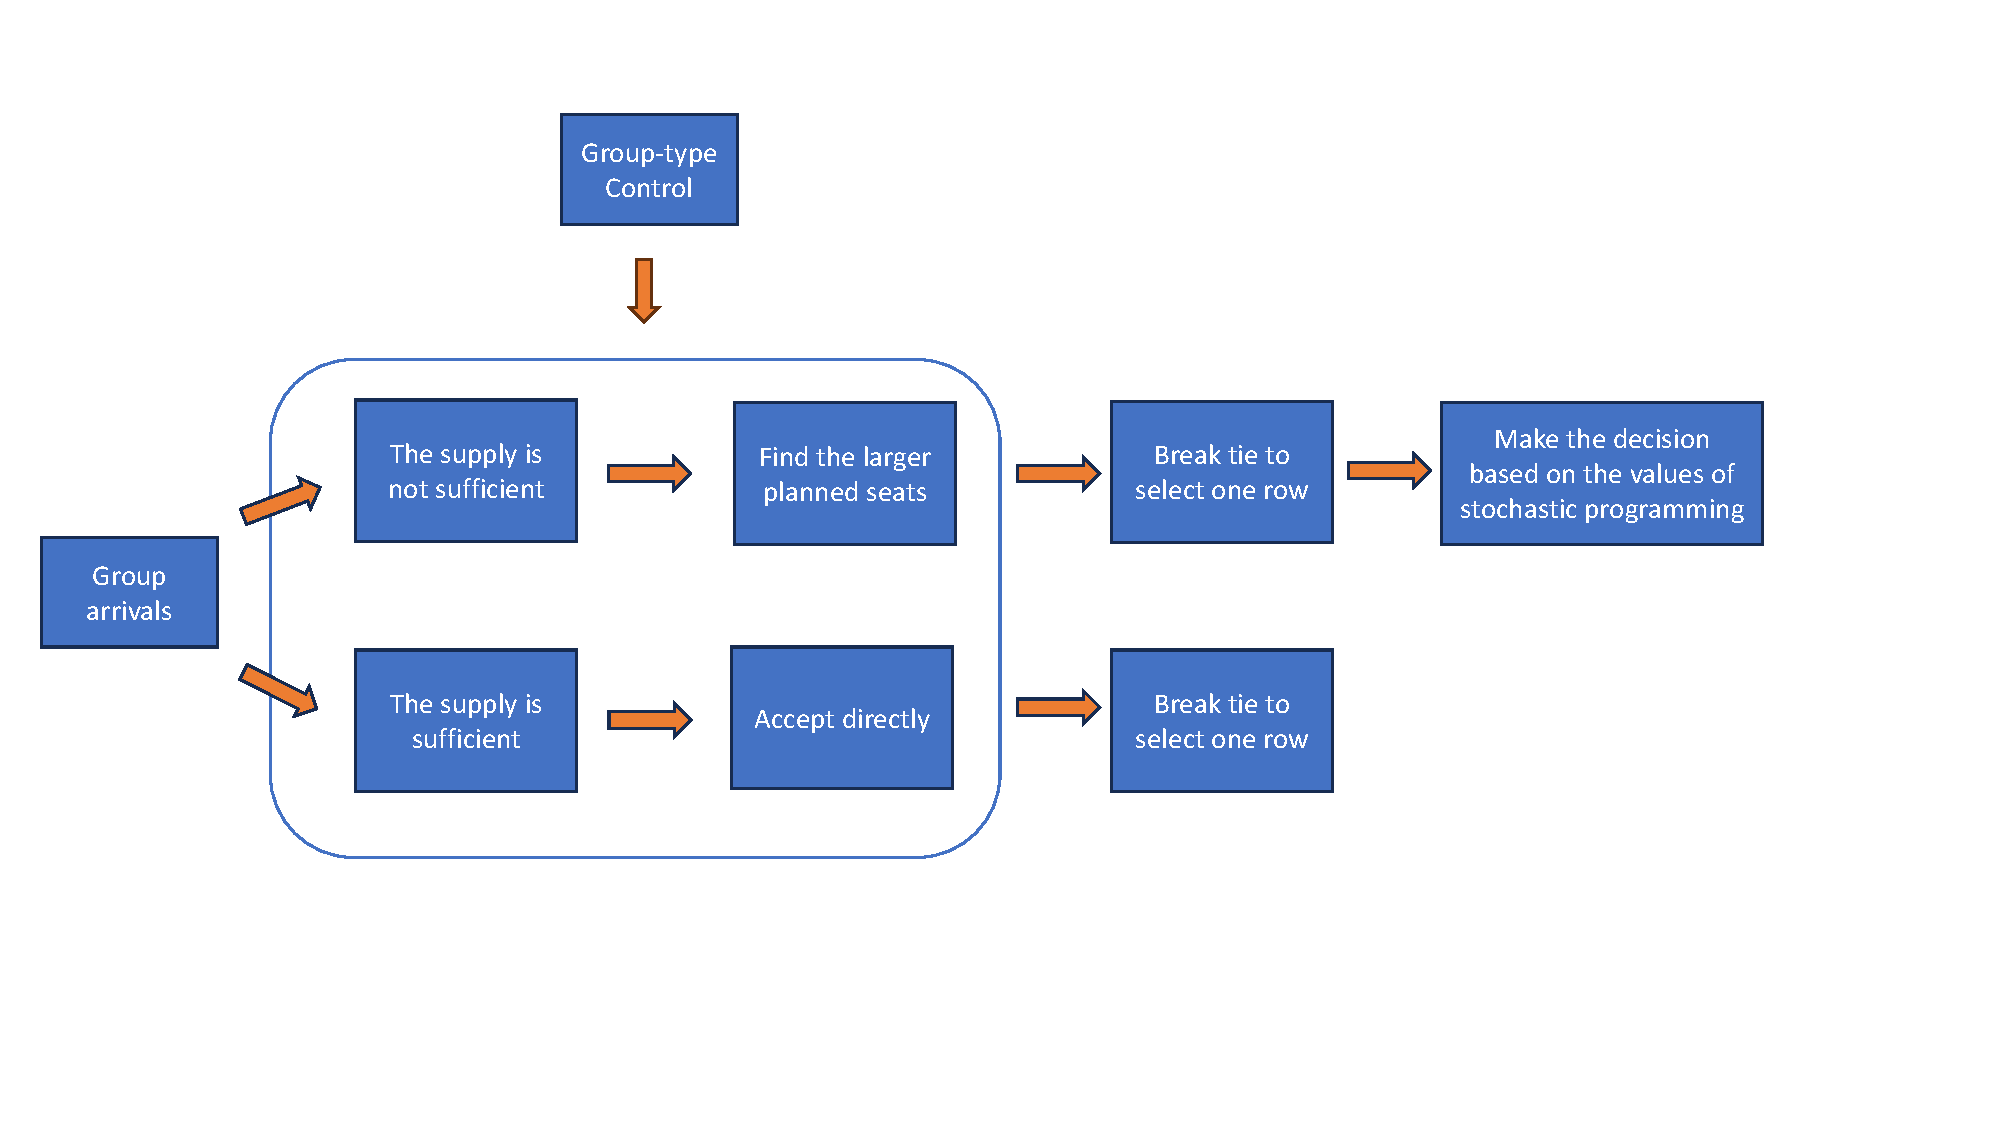
\includegraphics[width=1\textwidth]{./Figures/test.pdf}
% \end{figure}

\begin{algorithm}[H]
  \caption{Dynamic Seat Assignment}\label{algo_dynamic_policy}
  % \KwIn{Seat planning $\bm{H}$, Supply $\bm{X}$, $\mathbf{L}$}
  % \KwOut{Decision}
  \For{$t =1, \ldots, T$}
  { Observe group type $i$\;
    \eIf{$X_{i} > 0$}
    {Find row $k$ such that $H_{ki} >0$ according to tie-breaking rule\; Accept group type $i$ in row $k$, $L_{k} \gets L_{k} -n_{i}$\; $H_{ki} \gets H_{ki} -1$, $X_{i} \gets X_{i} -1$\Comment*[r]{Accept group type $i$ when the supply is sufficient}
    \If{$i = M$ and $X_{M} =0$}
    {Regenerate $\bm{H}$ from Algorithm 3\; Update the corresponding $\bm{X}$\Comment*[r]{Regenerate the seat planning when the supply of the largest group type is 0}}
    }
    {Calculate $d^{t}(i, j^{*})$\;
    \eIf{$d^{t}(i, j^{*}) >0 $}
    {Find row $k$ such that $H_{kj^{*}} > 0$ according to tie-breaking rule\; 
    Calculate the VoA under scenario $\Omega^{t}_{A}$ and the VoR under scenario $\Omega^{t}_{R}$\;
    \eIf{VoA $>$ VoR}
    {Accept group type $i$, $L_{k} \gets L_{k} - n_{i}$\; Regenerate $\bm{H}$ from Algorithm 3\; Update the corresponding $\bm{X}$\;}
    {Reject group type $i$\; Regenerate $\bm{H}$ from Algorithm 3\; Update the corresponding $\bm{X}$\;}}
    {Reject group type $i$\;}
    }}
\end{algorithm}




% \subsection{Break tie for Bid-price and DP base-heuristic}
% To determine which row to place accepted groups in when there are multiple options, follow these steps:

% 1. Check if the remaining capacity of the current row is greater than the maximum group size or equal to the current group size. If it is, accept the current arrival and place the group in that row.
% 2. Otherwise, consider the next row.
% 3. Repeat steps 3 and 4 until a row is found that can accommodate the current group size.


% \subsection{Seat Planning Charts Online}
% We are able to provide an online seat planning solution by using our method. For a feasible seating arrangement, we provide a pattern for each row. The sequence of groups within each pattern can be arranged arbitrarily, allowing for a flexible seat planning that can accommodate realistic operational constraints. Therefore, any fixed sequence of groups within each pattern can be used to construct a seating plan that meets practical needs.

% We need to assign seats to the group for each arrival. In each period, the group can select the row they want to sit when the capacity is enough. FCFS will be more appropriate. But M1 and M3 can also be used.


% update the scenario and the probability, add constraints when re-calculating stochastic programming.
% we can update the supply whenever some demand exceeds the supply.

% Then use Algorithm \ref{algo_nested_policy} to make the decision.


% \subsubsection{Ticket Reservation with Row Selection}
% There are two methods to achieve this goal.

% First, we can generate patterns planning according to stochastic information. Calculate the maximal supply from the mean demand. The supply gives the number of patterns with different losses; then we prepare the corresponding pattern planning for each row. Every group will be assigned in each period according to the designated row as long as the capacity allows. 

% The number of combinations is enormous.

% The second one is named the seat row selection method based on the stochastic seat assignment method. The initial supply is obtained from the stochastic model, then update the supply from the deterministic model after the first period. After accepting one group, we update the accepted demand and remaining seats. The policy follows section \ref{nested_policy}.


% Set the mean demand as the initial supply, update the supply from deterministic model by setting accepted demand as the lower bound. / can be used in scenario 1,2.


% Partially dynamic: at the beginning stage, the capacity is sufficient, thus we will accept all arrivals. 
% Multiple planning approach

% \subsubsection{FCFS-based}\label{FCFS-based}
% For dynamic seat assignment after all group arrivals, we can continue to use the first-come, first-served approach for seat assignment. Relax all rows to one row with the total number of seats. For each arrival, we need to check the feasibility of constructing a seat assignment in $N$ rows. If the seat assignment is feasible, we accept the request; otherwise, we reject it. The threshold capacity is $(L -u +1)$.

% find the target arrival when the number of seats taken by the preceding arrivals does not exceed the capacity.Then we obtain a new sub-sequence, including the arrivals from the first to the target and a possible arrival. 

% And use the nested policy to accept or reject one group in the remaining arrivals. 


% For the convenience of calculation, we check the feasibility of constructing a seat assignment from the end of the sub-sequence. When it is not feasible for the seat assignment, we should delete the group one by one from this sub-sequence until a feasible seat assignment is found. In reality, we need to check the feasibility one group by one.


% Each request will be assigned row by row. When the capacity of one row is not enough for the request, we arrange it in the next row. If the following request can take up the remaining capacity of some row exactly, we place it in that row immediately. We check each request until the capacity is used up. 


% There is a reservation stage, we only decide to accept or reject.
% After certain periods, there is a seat selection stage.

% Or use partial static information to estimate the probabilities, then generate new plannings.

% Multiple scenario approach:
% Suppose that we know the probabilities, we can use the sampling demands to estimate which patterns we should use. For example, three rows with $I_1$, seven rows with $I_2$. For each arrival, if there exists one scenario containing this group, we accept it; otherwise we use nested policy to accept or reject it.

% \subsubsection{Largest Patterns Planning}\label{largest_pattern}
% For each row, we choose the patterns from $I_1$. Accept the group such that the largest pattern can be maintained. When the arrival cannot be assigned in the planning patterns from $I_1$, we can change the largest pattern to a second largest pattern according to the coming arrival.


% \begin{lem}
%   Any largest patterns can be generated by the largest pattern constructed from the greedy method.
% \end{lem}

% This method can be used without stochastic information. The performance will improve when the total demand can construct the largest patterns for all rows.


% Once: Obtain the supply from the stochastic model by benders decomposition. Use the deterministic model to obtain a heuristi supply. Then use the multi-class rule to decide whether to accept the group at each period.

% Several: Initially, set the mean demand for all periods as the upper bound of demand. Then obtain the supply from the deterministic model. Set the accepted demand as the lower bound of demand, the upper bound of demand will be the sum of accepted demand and mean demand for the remaining periods. Update the lower bound and upper bound when some supply runs out.

% One counterexample: [15,21,13,3] /[15,21,10,3]  reject 4

% Different types of movies will have different probabilities, consider the preference for policy when demand = supply.


% The numbers in the `performance compared to the optimal' represent M1, M2, M3, M4, M5, M6 respectively in order.

% The maximal number of people served can be obtained by \eqref{deter_upper} with a realized sequence of arrival.

% Some important information:
% The government will give the restriction: 入座人数50% /相连座位 4个

